\setchapterpreamble[o]{%
  \dictum[Lao-tzu]{\textit{``A journey of a thousand miles begins with
      a single step.''}}}

\chapter{Fundamentals}
\label{cha:fundamentals}

This chapter  provides you  with the description  of basic  principles and
concepts  that have  been  used in  this  work. The  chapter is  basically
separated into two  parts: Concepts that have already  been pointed out in
the  previous  chapter  and  descriptions  of technologies  that  lead  to
important design decisions.

The  first part  starts  with an  introduction  into the  \emph{Extensible
  Markup Language}. \gls{glo:XML} is the description language that is used
for  the  \emph{Job  Submission  Description  Language},  the  \emph{Basic
  Execution Service}  and the messages  which are used in  the implemented
communication  protocol  (see Section~\ref{sec:communication-protocol}  on
page \pageref{sec:communication-protocol}).

The second and last part of this chapter provides the reasoning which lead
to  the decision  to base  the \gls{glo:XenBEE}  on  an \emph{asynchronous
  message-passing  communication  model}.    It  also  discusses  how  the
communication between the distributed components can be secured.

\section[The Extensible Markup Language]
{The Extensible Markup Language (\gls{glo:XML})}
\label{sec:fundamentals:xml}

The Extensible Markup Language \cite{xml}  is a simple, yet very flexible,
plain text based description format. The format represents a subset of the
\emph{Standard  Generalized Markup Language}  (SGML).  It  can be  used in
variety of ways  and even more usages are discovered  still. Usages of XML
can be found in  \emph{XHTML}, \emph{RSS}, \emph{Atom}, \emph{Math-ML} and
many more.   Due to the  structured semantics of  XML, more and  more file
formats are  nowadays based  on XML,  thus replacing the  old INI  or Unix
\texttt{rc}  files  ---  a very  popular  example  in  this field  is  the
\emph{OASIS  Open Document  Format for  Office Applications}\footnote{More
  information   about  the   Open  Document   Format  can   be   found  on
  \url{http://www.oasis-open.org/committees/tc_home.php?wg_abbrev=office}}.

An XML-file is  an ordinary plain text file, that  could have been created
by any text  editor.  The most important building  blocks of XML-files are
\emph{elements}, \emph{attributes} and \emph{text}.

Elements   are  \emph{logical  structures},   that  can   have  additional
attributes and  sub-elements or \emph{children}, whereas  the children can
either be other elements or text.  The following example shows you a small
XML document. Every XML  document contains \textbf{exactly one} designated
\emph{root} element, which is simply the first element in the document.

For parsing purposes,  an XML document can be represented  as a tree, this
is  shown in Figure~\ref{fig:xml-example}.   A widely  used model  for the
in-memory  representation of  XML documents  is the  \emph{Document Object
  Model} (DOM).  Most  of the available XML parsers,  provide an interface
for parsing a document into  an in-memory representation that follows this
model. The programmer  can then simply add, delete  or modify elements and
attributes by  using an object-oriented  interface.  Using the  example in
Figure~\ref{fig:xml-example}, a programmer could for instance iterate over
all children  of the \texttt{root}-element, that have  a tagname (\ie the
name  of the  element) equal  to ``child''  --- in  this case,  that would
result in just two elements.

\begin{figure}[h]
  \centering
  \begin{tabular}{rc}
    \begin{minipage}[c]{.35\textwidth}
      \begin{lstlisting}[language=XML]
<root foo="bar">
  <child/>
  Some text
  <child>More text</child>
</root>
      \end{lstlisting}%
    \end{minipage} &
    \begin{minipage}[c]{.35\textwidth}
      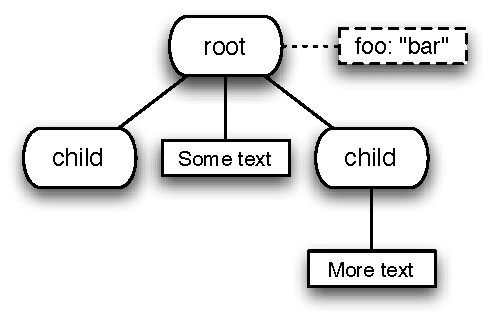
\includegraphics[width=5cm]{xml-example}
    \end{minipage}
  \end{tabular}
  \caption{A simple XML example}
  \label{fig:xml-example}
\end{figure}

\subsection{Namespaces}

XML  documents   may  contain  elements  and   attributes  from  different
vocabularies (\ie different document  types). To resolve ambiguity between
the  involved   vocabularies,  the  W3C  recommends  the   use  of  unique
\emph{Namespaces}  that are  assigned  to each  element.   A document  may
contain a  \emph{default}-namespace to which  all elements belong  that do
not  have  a  special  namespace  assigned.   Within  a  single  document,
namespaces are given  a logical name. The logical  name itself is assigned
the unique Namespace identifier (\eg a \gls{glo:URI}). Some namespaces and
common   ``names''   for  them   are   given   in   the  following   table
(Table~\ref{tab:namespaces}):

\medskip

\begin{table}[ht]
  \centering
  \begin{tabular}{@{}ll@{}}\toprule
    logical name        & \multicolumn{1}{l}{namespace URI} \\ \midrule % header
    \texttt{xsd}        & \url{http://www.w3.org/2001/XMLSchema} \\
    \texttt{jsdl}       & \url{http://schemas.ggf.org/jsdl/2005/11/jsdl} \\
    \texttt{jsdl-posix} &  \url{http://schemas.ggf.org/jsdl/2005/11/jsdl-posix} \\
    \texttt{dsig}       & \url{http://www.w3.org/2000/09/xmldsig#} \\
    \texttt{bes}        & \url{http://schemas.ggf.org/bes/2006/08/bes-activity} \\
    \texttt{xbe}        & \url{http://xenbee.berlios.de/schemas/xbe/2007/01/xbe} \\
    \texttt{xbe-sec}    & \url{http://xenbee.berlios.de/schemas/xbe-sec/2007/01/xbe-sec} \\
    \texttt{xsdl}       & \url{http://xenbee.berlios.de/schemas/xsdl/2007/01/xsdl} \\
    \bottomrule
  \end{tabular}
  \caption[XML Namespaces used in this work]{Important namespaces}
  \label{tab:namespaces}
\end{table}

Namespaces  are   specified  in  the  XML  using   the  special  attribute
\texttt{xmlns}.     An   attribute    of   an    element,    which   reads
\texttt{xmlns="www.example.com"}, sets the  default namespace to the given
URI, while  \texttt{xmlns:foo="www.example.com"} makes the  same namespace
known as the logical name  ``foo''. In another document the same namespace
could have been assigned the logical name ``bar'' as well.

To specify  that a  given element  belongs to a  namespace other  than the
default namespace, the  element's name is prefixed by  the logical name of
the namespace,  \eg \texttt{foo:child} means, that  the ``child'' element
belongs to the namespace defined by ``foo''.

\subsection{Validation of XML documents}
\label{sec:xml-validation}

A  really nice  and very  useful  addition to  XML is  the possibility  to
\emph{validate}  an XML  document.  There  are two  mechanisms  to provide
validation,    the    \emph{Document    Type   Definition}    (DTD)    and
\emph{XML-Schema}.

\subsubsection{Document Type Definition}

A DTD defines for a particular  document what elements are allowed and how
their attributes look like. The  composition of elements to form container
(\ie parent)   elements  can   be   described  in   a  rudimentary   way.
Unfortunately, the  DTD uses  its own syntax,  that has nothing  in common
with  the syntax of  an XML  document. For  an author  of an  XML document
type\footnote{for example the configuration file format of an application}
that means in particular, that he has to learn two different syntaxes.

\subsubsection{XML-Schema Definition}

XML-Schema is  itself defined  using XML as  its description  language and
obsoletes the  DTD. It is much  more powerful, for instance,  an author is
able  to   restrict  the   actual  data  an   element  or   attribute  may
contain.  Let's for  instance  say, a  given  attribute can  only take  on
non-negative  integers.    To  reflect  this  constraint   in  the  schema
definition,  the   author  would  set   the  type  of  the   attribute  to
\texttt{xsd:nonNegativeInteger}.

There are many predefined data types, an author may use to create new data
type constraints.  An XML-Schema validator complains, if  a document, that
is  supposed to  conform  to  that schema,  contains  the just  introduced
attribute with a negative value, \eg $-1$.

The advantages of XML-Schema over a DTD are obvious.  When using DTDs, the
application  itself was  responsible to  check  the validity  of each  XML
document  that it  used.  That  means, the  same functionality  had  to be
implemented over and over again, \ie  each time a new application wants to
make use of a given XML document type. While using XML-Schema definitions,
the author of  an XML document type defines  the validity constraints just
once and any application  may rely on that.

To make that clear, here is a short example: Suppose there is a definition
for  an  element  called  ``\texttt{entry-id}''  which may  only  take  on
positive integer values.  Since a DTD does not support constraints on data
types, each  application must check for  itself if the  value matches that
type.  Now suppose the constraint for  that element is changed so that the
number $0$  is included  as well ---  in each application,  the validation
code must be modified to match the new constraint.

\section[The Job Submission Description Language]
{The Job Submission Description Language (\gls{glo:JSDL})}
\label{sec:fundamentals:jsdl}

\gls{glo:JSDL} is a very extensible XML-based description language for the
submission  of computational  jobs \cite{jsdl-spec}.   With \gls{glo:JSDL}
you are  able to  describe all requirements  that a computational  job may
need for the submission to a remote resource --- mainly the \gls{glo:JSDL}
addresses grid resources but it is not limited to that.

Nearly  every  element of  the  \gls{glo:JSDL}  specification may  contain
arbitrary  many  user-defined  elements  from  other  XML  specifications.
Therefore  is  the JSDL  adoptable  to  upcoming  user requirements.   The
\gls{glo:JSDL} has been  extended in this work to  support the description
of   virtual  machines   (see   Section~\ref{sec:xen-based-submission}  on
page~\pageref{sec:xen-based-submission}).

To explain  this, consider the  following example. To  execute a job  on a
resource  a previously  acquired  reservation is  required.   To add  this
information  to the job  submission, the  \gls{glo:JSDL} would  include an
additional   element   which   holds   all   information   regarding   the
reservation. Such extension elements  are purely optional and systems that
are unaware of a particular extension element may just neglect it.

The following section roughly describes the most important components that
are needed to form a useful submission description.

\subsection{``Hello World'' with the JSDL}

A    \gls{glo:JSDL}    document     does    always    start    with    the
\texttt{JobDefinition} element,  which is the top-level  element and holds
all required information about the job.

Let's assume a user wants to execute a small program on a remote resource.
The  program  will  indeed be  very  simple,  it  just prints  the  string
``\texttt{Hello World}'' to its  standard output stream.  The execution of
this application on the user's local computer could be similar to:

\begin{minipage}{0.75\textwidth}
  \begin{lstlisting}[language=ksh]
    $ echo "Hello World"
    Hello World
    $
  \end{lstlisting}
\end{minipage}

This  excerpt  represents  the   execution  in  a  standard  UNIX  command
shell. Note that the \texttt{echo}  program does nothing more than writing
the parameters passed to it to its \texttt{stdout} stream. Now suppose the
user  desires  to execute  the  same program  on  a  remote resource.  The
\gls{glo:JSDL}  document will  look somewhat  like the  document  shown in
Listing~\ref{lst:jsdl-example}.

\medskip
\begin{center}
%  \begin{minipage}{.75\textwidth}
    \begin{lstlisting}[captionpos=b,float=t,backgroundcolor=\color{listingcolor},frame=lines,numbers=none,stepnumber=5,numberfirstline=false,numberstyle=\tiny,caption={A
      small ``Hello World''-example written in
      \gls{glo:JSDL}},label={lst:jsdl-example},language=XML]
<jsdl:JobDefinition>
 <jsdl:JobDescription>
    <jsdl:Application>
      <jsdl-posix:POSIXApplication>
        <jsdl-posix:Executable>
          /bin/echo
        </jsdl-posix:Executable>
        <jsdl-posix:Argument>Hello World</jsdl-posix:Argument>
      </jsdl-posix:POSIXApplication>
    </jsdl:Application>
  </jsdl:JobDescription>
</jsdl:JobDefinition>
     \end{lstlisting}
%   \end{minipage}
\end{center}

Note, that  the shown \gls{glo:JSDL}  document describes exactly  the same
execution  the  user  had  previously  performed  locally.   The  executed
\texttt{echo} program  again writes  its arguments to  its \texttt{stdout}
stream.   Different from the  local execution  is in  this case,  that the
output will  be lost, since the user  did not specify what  should be done
with the  generated output.  If the  user was interested  in the program's
output, he  had to specify  the redirection of  the output stream  to some
file  and a  staging operation  that transfers  the created  file  to some
location he has access to.

\subsection{Important elements}

A typical \gls{glo:JSDL} document consists  of the following parts --- job
identification,  application description,  resource descriptions  and data
staging elements. To keep the example simple, only the second one has been
used in the example  in Listing~\ref{lst:jsdl-example}.

\subsubsection{Job identification}

The \texttt{JobIdentification}  element is used to  hold information about
the job, such as a descriptive  name, that is mostly interesting for human
beings.  Nonetheless it  may hold additional information that  could be of
interest to  applications processing the document ---  such as annotations
(\eg a  unique task  identification number  could  be stored  in such  an
annotation).

\subsubsection{Application}

With the \texttt{Application} element, a user describes the program itself
---  \ie the  real executable,  that  is going  to  be  used.  A  special
extension --- \texttt{POSIXApplication}, also defined in the specification
\cite{jsdl-spec}   ---   can  be   used   to   describe  executables   for
\gls{glo:POSIX}-compliant   operating  systems  \cite{posix}.    You  have
already      seen     the     usage      of     this      extension     in
Listing~\ref{lst:jsdl-example},  where it  had  been used  to specify  the
execution of the \texttt{echo} command line program.

\subsubsection{Resources}

This element can be used  to describe various resource requirements of the
application. Some of the many resource types one can use are listed below.

\begin{itemize}
\item the number of CPUs the job requires
\item the operating system required by the job
\item amount of virtual memory that must be available for the job
\item file-systems  and their expected  mount-points
\end{itemize}

All  specified file-systems  must  be  made available  for  the job  prior
execution. Every file-system specification  defines a unique name that can
be used to refer to that particular file-system in other elements, such as
staging operations.  Thereby the  user can define \emph{logical names} for
special directories within the execution environment of the task.
  
\subsubsection{Staging operations}

The   \texttt{DataStaging}    element   is   used    to   define   staging
operations.  These operations  can either  be  \emph{Stage-In} operations,
which  refer  to files  that  have to  be  transfered  into the  execution
environment  prior   the  execution  of  the   task,  or  \emph{Stage-Out}
operations, which refer  to transfers that have to be  made after the task
has been executed.

A user may  specify the \texttt{DataStaging} element as  often as he likes
to.   The most  relevant elements  within  a staging  instruction are  the
\texttt{Source}  and \texttt{Target}  elements, both  of them  can  hold a
\texttt{URI}  element  to  specify  a  generic  location.   The  mandatory
\texttt{FileName} element points to  an actual file within the file-system
hierarchy of the execution environment of the task. The actual location of
a file can be given relative  to a previously defined file-system, in this
case the \texttt{FilesystemName} element must be specified and is required
to contain the logical name of \texttt{FileSystem} resource.

\subsubsection{Conclusions}

The \gls{glo:JSDL}  is a  powerful description language  for computational
jobs. It aims  to cover the description of the  job submission for typical
computational  jobs. The \gls{glo:XenBEE}  is such  an example,  since the
\gls{glo:JSDL}  does not  know anything  about executing  jobs  on virtual
machines.  The extensions  to the \gls{glo:JSDL} that I  have designed and
implemented  are   covered  in  Section~\ref{sec:xen-based-submission}  on
page~\pageref{sec:xen-based-submission}.

The  next  section  deals  with  the  \emph{Basic  Execution  Service},  a
specification that  provides a common execution  semantic of computational
jobs. This semantic is backed  up by an extensible state-model to describe
the job execution.

\section[The Basic Execution Service]{The Basic Execution Service (BES)}
\label{sec:fundamentals:bes}

The \emph{Basic Execution Service} \cite{ogsa-bes} is a specification that
defines  a service  (\eg a  web service)  which provides  functionality to
control \emph{Activities}.  An \emph{activity}  can be seen as an abstract
view on a computational job. A user  is able to submit an activity to the
execution service and  can later on control and  monitor that activity ---
using web service calls, for instance.

Control  of  the  activity  is   basically  limited  to  a  request  which
\emph{terminates} the  activity. The monitoring of an  activity results in
returning the activity's current state.

The state  of an activity is  modeled using a finite  state automaton. The
specification  of  the  \gls{glo:BES}  incorporates  a  simple,  but  very
extensible, state  machine for  activities. It comprises  a total  of just
five  states  an  activity  can  be  in  at  any  time:  \texttt{Pending},
\texttt{Running},       \texttt{Finished},       \texttt{Failed}       and
\texttt{Terminated}. 

To be extensible and integrable  into existing environments, the states of
the \gls{glo:BES}  are represented using a XML  specification. The element
which   represents   the  current   state   of   an   activity  is   named
\texttt{ActivityStatus} and belongs to  the \emph{bes} namespace as it has
been  defined  in Table~\ref{tab:namespaces},  the  state  itself is  then
specified using the \texttt{state} attribute:

\begin{lstlisting}[language=XML]
  <bes:ActivityStatus state="Running"/>
\end{lstlisting}

The    basic    state   machine,    or    state-model,    is   shown    in
Figure~\ref{fig:bes-basic}. To  reflect the request for  termination of an
activity, each  non-terminal state provides an outgoing  transition to the
\texttt{Terminated} state.

\begin{figure}[h]
  \centering
  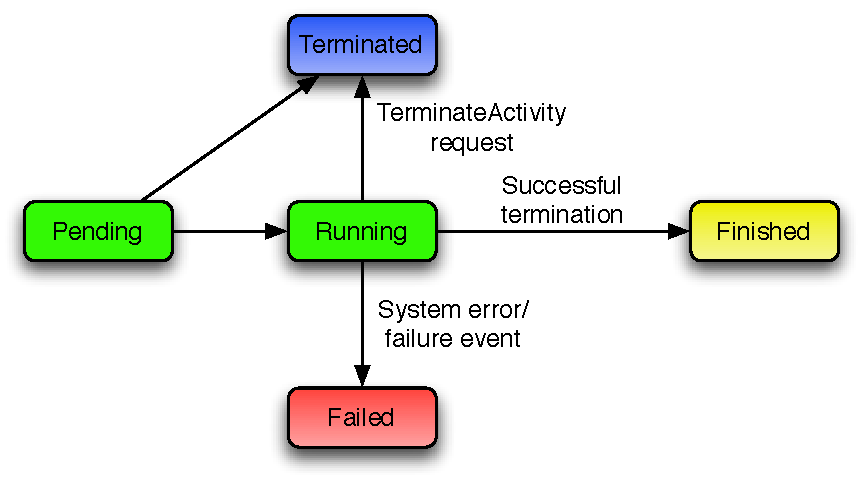
\includegraphics[scale=.6]{bes-basic-job-model}
  \caption[Basic BES Job-State-Model]{This is the job-state-model as it is
    defined in the BES specification \cite{ogsa-bes}}
  \label{fig:bes-basic}
\end{figure}

This  basic state-model  represents everything  a possible  client  of the
execution service needs  to know. An actual execution  service may require
to  use  additional  states.   It  can  define both  new  states  and  new
transitions,  as  long  as  it  conforms  to a  rather  simple  rule:  the
\textbf{visual behavior}, as it is experienced by some client, must not be
altered. A breakage of this rule would be the introduction of a transition
from  the \texttt{Running}  state  back into  the \texttt{Pending}  state.
Clearly, the visual behavior a  client experiences, has changed, since the
client  simply  does   not  expect  that  the  activity   is  suddenly  in
\texttt{Pending} again.

\subsection{Extending the state-model}

New  states can  be added  by  splitting up  either one  of the  ``basic''
states, or  a state that is  an extension itself.   Among these sub-states
any number  of new transitions  may be introduced.  The  following example
for  an extension  has  been taken  from  the \gls{glo:BES}  specification
\cite{ogsa-bes}.

Suppose the execution service provides  a way to suspend a given activity.
This  requires  not only  additional  user  requests  --- one  to  request
\emph{suspension} and  one to request  \emph{resumption} --- but  also two
new states. These states are modeled as sub-states of the \texttt{Running}
state, since an  activity may only be suspended  while it already running.
The  \texttt{Running} state is  now internally  split into  the sub-states
\texttt{Executing} and \texttt{Suspended}.   The extended state machine is
shown in Figure~\ref{fig:bes-suspend-model}

\begin{figure}[h]
  \centering
  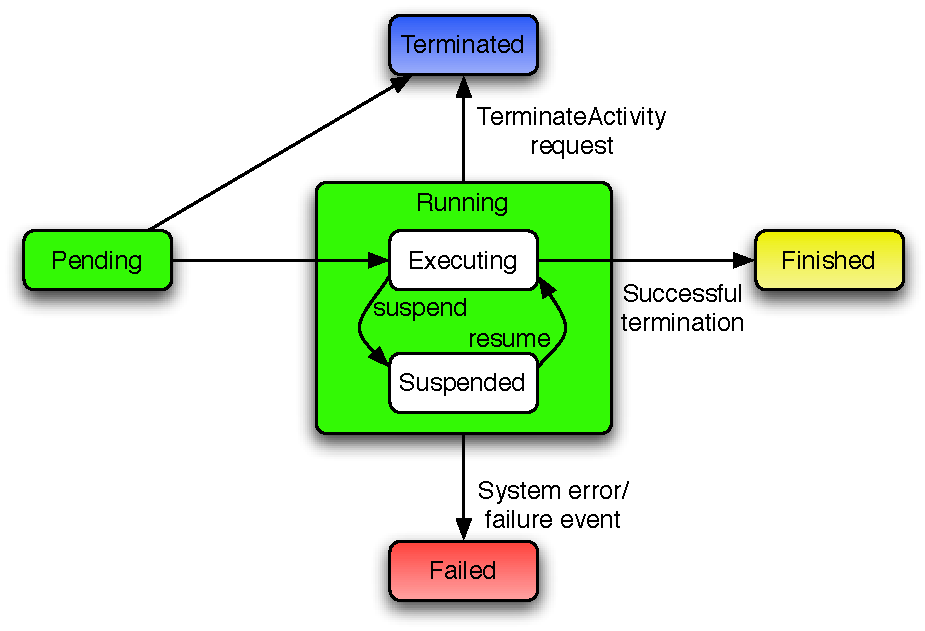
\includegraphics[scale=.6]{bes-suspend-job-model}
  \caption[Extended  BES Job-State-Model]{The  basic state-model  has been
    extended  to  support suspension  (taken  from  the BES  specification
    \cite{ogsa-bes}).}
  \label{fig:bes-suspend-model}
\end{figure}

The nice  thing about  the extensibility of  this state-model is  that any
client that ``understands'' the  basic model, will understand any extended
model as well. That is  because the \emph{visual behavior} does not change
and  therefore  will never  ``anything  unexpected''  happen. This  visual
behavior is  directly reflected  in the XML  specification of  the current
state.  Any  additional states are represented  by user-definable elements
added  to  the  \texttt{ActivityStatus}  element as  sub-elements.   Let's
assume  the just modeled  extension defines  its own  state representation
using its own namespace.  The  current state of a suspended activity could
then be written as:

\begin{lstlisting}[float={h!},language=XML]
  <bes:ActivityStatus state="Running">
     <ext:Suspended/>
  </bes:ActivityStatus>
\end{lstlisting}

The state is still \texttt{Running}, but  any client that is aware of this
extension   will  know   how  to   interpret   the  \texttt{ext:Suspended}
sub-element, \ie it could provide  a user with the possibility to resume
the action.

The state-model  that is  used by the  \gls{glo:XenBEE} extends  the basic
model  with  support  for  staging operations,  reservations  and  virtual
machines,  it   can  be  found   on  page~\pageref{sec:xbed:job-model}  in
Section~\ref{sec:xbed:job-model}.

This section closes the description of the technologies that were required
for  the \gls{glo:XenBEE}  to provide  batch job  execution  semantics and
integrability into grid-environments.  The following sections motivate the
applied communication model and how  this model can be enhanced to provide
secure communication.

\section{Communication Model}
\label{sec:fundamental:communication-model}

Communication in distributed systems  can be either \emph{synchronous}, or
\emph{asynchronous}  \cite{MeCa:2005:Taxonomy}.   This section  summarizes
these two models and results  in the definition of the communication model
used by the \gls{glo:XenBEE}.

\subsection{Programming Models}

The programming model of  synchronous communication is called \emph{Remote
  Procedure Calls}  (RPC, \cite{rpc}). It provides the  same function call
semantics as a local function call, \ie the program waits until the result
is   computed  and  returned   by  the   remote  system.    Commonly  used
implementations of  this model are the \emph{Common  Object Request Broker
  Architecture} (CORBA, \cite{corba}), the \emph{Remote Method Invocation}
(RMI, \cite{rmi}) or the  \emph{Distributed Component Object Model} (DCOM,
\cite{dcom}).

Asynchronous   communication  follows   the  emerging   paradigm   of  the
\emph{event-based   communication  model}   \cite{MeCa:2005:Taxonomy}.   A
request  that is  sent  to a  remote  system does  not  have an  immediate
result. The  result, if any, is  received by the  caller asynchronously to
his current computation. The  distributed components that use asynchronous
communication  are interconnected  by  using message-passing  technologies
such as the \emph{Message Passing Interface} (MPI, \cite{mpi}).

The  \gls{glo:XenBEE}  can be  implemented  using  either  of two  models.
Consider for  example the request for  the termination of  a submitted job
using a single-threaded client application. The client could make a remote
procedure call  and wait until the  termination has been  performed on the
remote site.   Or the client just sends  the request to the  server and is
able to accept further input from the user.

The   \gls{glo:XenBEE}  will   be   designed  to   use  the   asynchronous
communication  model.    This  implies   the  use  of   a  message-passing
technology.

\citet{dad-mom}  state, that:
\begin{quotation}
  \emph{``Every  DAD  (Distributed  Application  Developer)  needs  a  MOM
    (Message Oriented Middleware)''}.
\end{quotation}


\subsection[Message Oriented Middleware]{Message Oriented Middleware (MOM)}
\label{sec:fundamentals:mom}

Message-passing in  distributed systems need  not be based on  direct (\eg
\gls{glo:TCP}) connections between each component. The messages can easily
be transmitted to an intermediate system which forwards the message to the
target  system.   This section  describes  a  middleware component  called
\emph{Message-Queue Server} (\gls{glo:MQS}) which can be used in this kind
of distributed systems to improve communication quality.

The abstraction  from direct connections  between each component  leads to
the definition  of \emph{logical connections}.  A logical  connection is a
connection between distributed components that pass messages to each other
while not being directly connected to each other.

To send a message to some component using logical connections, the message
is addressed to  a logical destination and sent  to an intermediate server
that hopefully  knows the  actual target. To  receive messages  from other
components, a component registers itself with the intermediate server.

Such   an   intermediate   server   is   a   \emph{Message-Queue   Server}
(\gls{glo:MQS}). The  protocol layers  that are involved  when application
data is  to be transmitted from  one component to another  are depicted in
Figure~\ref{fig:mqs-layers}.

\begin{figure}[ht]
  \centering
  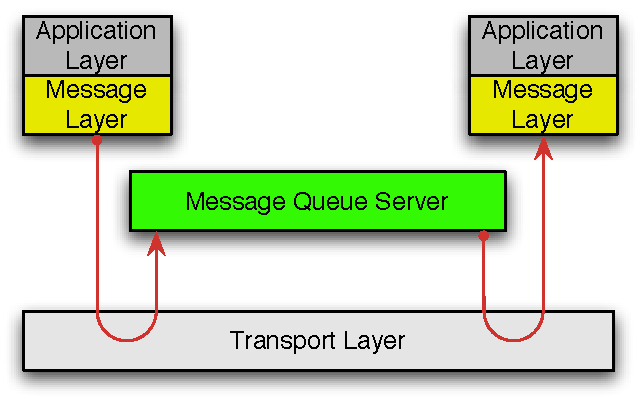
\includegraphics[scale=0.7]{mqs-layers}
  \caption{Protocol layers in an \gls{glo:MQS}-based communication.}
  \label{fig:mqs-layers}
\end{figure}

The  usage of  such an  intermediate \gls{glo:MQS}  has  several important
advantages over direct connections between the distributed components:

\begin{itemize}
\item All  messages are sent to \textbf{logical  queues} (\ie end-points).
  This means that  the details of the connection of  a remote component is
  hidden to other components.  For  example, the IP address of a component
  may  change between  two subsequent  messages sent  to it  without being
  noticed by the sender.
\item All  connections are \textbf{outbound} which  effectively means that
  all  components  may  reside   behind  a  (restrictive)  firewall  or  a
  \gls{glo:NAT}-gateway.   This not  only  increases the  security of  the
  \emph{xbed},   but    also   targets   the    problems   which   typical
  network-policies     and    hence    resulting     network-layouts    of
  grid-environments or companies impose.
\item The  \gls{glo:MQS} need not  to be on  a single machine, but  can be
  distributed  over  many computers  to  implement \textbf{fail-over}  and
  \textbf{load-balancing}.
\item Messages  can be  kept in a  \textbf{consistent storage}  within the
  \gls{glo:MQS} if they  cannot be delivered right now.   That may happen,
  if the communication partner is temporarily disconnected --- all pending
  messages will be delivered as soon as the end-point connects again.
\item    Multiple   \gls{glo:MQS}   can    be   configured    to   provide
  \textbf{forwarding and  routing} of  messages destined for  a particular
  queue --- that means independence from the actual network-topology.
\item A \gls{glo:MQS} can be configured to provide \textbf{authentication}
  and \textbf{authorization} to limit access to particular queues.
\item   Messages   sent   from   one   component   to   another   can   be
  \textbf{transformed}  while passing  the \gls{glo:MQS}.   That  means in
  particular,  that each  component may  send messages  in its  own native
  format and the \gls{glo:MQS}  intelligently transforms the messages into
  the native format of the receiver.
\end{itemize}

The drawbacks  of the  usage of \gls{glo:MQS}  are: An increased  delay in
message  transmission,  because all  messages  must  be  processed by  the
\gls{glo:MQS}  before they  can be  delivered.  And  that the  secure (\ie
encrypted)  transmission  of  messages   has  to  be  implemented  by  the
applications themselves.  The latter issue is discussed in more detail and
with        regard         to        the        \gls{glo:XenBEE}        in
Section~\ref{sec:secure-communication}.

\begin{figure}[htbp]
  \centering
  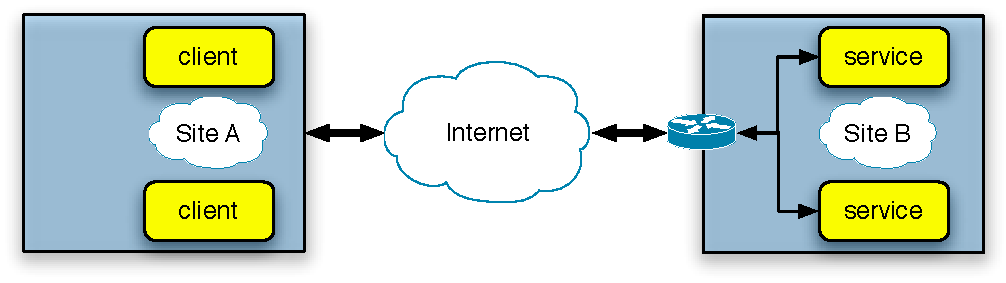
\includegraphics[scale=.75]{mqs-topology}
  \caption[Example  MQS topology]{A simple  message-based system  which is
    using a \gls{glo:MQS}.}
  \label{fig:mqs-topology}
\end{figure}

An example for a distributed system  that uses a \gls{glo:MQS} is shown in
Figure~\ref{fig:mqs-topology}.  Site~$B$ has  some services connected to a
\gls{glo:MQS}.   These services can  be reached  by clients  from site~$A$
through an  internet connection.  The  steps involved in building  up this
communication scheme are:
\begin{enumerate}
\item  Each service  connects to  the \gls{glo:MQS}  and \emph{subscribes}
  itself to a unique queue (\eg service.\emph{X}).
\item    Clients   subscribe    themselves   to    unique    queues,   too
  (\eg client.\emph{Y}).
\end{enumerate}

Now  that each  party is  subscribed to  its own  unique queue,  a two-way
communication is possible:
\begin{enumerate}
\item A client  that wants to communicate with one  of the services, sends
  its messages  to the unique queue  of that particular  service. The sent
  message  contains a  special \emph{reply-to}  field that  is set  to the
  unique queue of the client
\item Answers from  a service to a connected client are  sent to the queue
  specified in the reply-to field of received messages.
\end{enumerate}

The same  communication scheme  will be used  in the  \gls{glo:XenBEE}, as
well.  Each  component subscribes  itself to a  unique queue,  whereas the
queue of the \emph{xbed} will be configurable by an administrator.

The  next section  describes how  the message-based  communication  can be
secured, \ie  eavesdropping, modification and forgery of  messages must be
prevented.

\section{Secure Communication}
\label{sec:secure-communication}

Since the proposed system uses message queues to transfer messages between
clients  and  the   server,  all  transmitted  messages  are   sent  to  a
message-queue server  first. If  this intermediate server  is compromised,
all messages that pass through it can also be read by the intruder.

There are  two different  approaches to ensure  a secure transport  of the
messages from a  client to a server and  vice versa: \emph{Transport Layer
  Security} (TLS, \cite{rfc2246})  and \emph{Message Layer Security} (MLS,
\cite{mls, oasis-wss}). 

Both of them use public-key certificates, \eg \gls{glo:X509} certificates.
A public-key certificate is a data  structure that binds a public-key to a
subject (person  or system)  \cite{rfc2459}. If a  communication is  to be
secured by the use of public-key certificates, the ``users of a public-key
must be confident that the associated private-key is actually owned by the
correct  remote subject''  \cite{rfc2459}.   This can  be accomplished  by
having a trusted authority  digitally sign the involved certificates. Such
an infrastructure  is a called  a \emph{Public Key  Infrastructure} (PKI).
More   information  about   public-key  cryptography   can  be   found  in
Appendix~\ref{app:sec:public-key-cryptography}                           on
page~\pageref{app:sec:public-key-cryptography}.

The following  section describes  the \emph{Public Key  Infrastructure} in
detail.  After that the  \emph{Transport Layer Security} and \emph{Message
  Layer  Security} protocols  are discussed  and analyzed.   Subsequent to
that the implications for the \gls{glo:XenBEE} are discussed.

\subsection[Public Key Infrastructure]{Public Key Infrastructure (PKI)}

A  \emph{Public Key  Infrastructure} provides  the authentication  of user
identities using  public-key certificates.  The main aspect  is that there
are special \textbf{trusted  third parties} (\emph{Certificate Authority},
\gls{glo:CA})  that   are  permitted  to   \textbf{digitally  sign}  other
certificates. If a user\footnote{or some server, etc.}  wants to prove his
identity to  another entity, his  certificate is validated by  that entity
against the CA's certificate.  If the validity could be verified, the user
successfully proved that he is  in possess of the private-key that belongs
to this public-key \cite{rfc2459}.

The \gls{glo:CA} is responsible for checking that the public-key contained
in  the certificate  actually belongs  to the  requesting user,  server or
other  entity denoted  in the  certificate.  This  process is  for example
performed by verifying the credentials of a user (\eg with help of a photo
identification).

Any third-party that trusts a given CA will transparently trust any entity
that offers a certificate signed by that particular CA.

Validation is performed by verifying  that the certificate itself has been
signed  by a  trusted authority  --- the  actual validation  process  is a
little   bit  more  complex,   since  it   involves  checking   against  a
\emph{Revocation List} and  a ``best before'' date (\ie life  time of the
certificate), too.

The  signing  process  uses  the  authority's private  key  to  compute  a
cryptographic signature. This private-key must of course be kept in a very
secure  location  (\eg on a  physically  from  the Internet  disconnected
computer) ---  if it would fall into  the wrong hands, the  whole chain of
trust is compromised.

\begin{figure}[h]
  \centering
  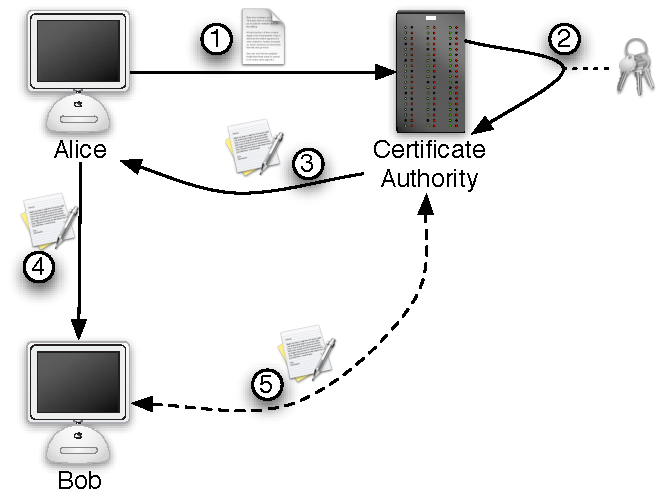
\includegraphics[scale=.55]{pki}
  \caption[Public  Key Infrastructure]{Alice  proofs her  identity  to Bob
    using a certificate  that is signed by a CA that  both, Alice and Bob,
    trust.}
  \label{fig:pki}
\end{figure}

An  example verification  process  is shown  in Figure~\ref{fig:pki},  the
steps can be described as follows:
\begin{enumerate}
\item \emph{Alice} request the signing of her certificate by a CA and thus
  sends a certificate request to the CA containing her public-key.
\item The CA in turn verifies Alice's credentials and eventually signs the
  certificate with its private key.
\item The signed certificate is sent back to \emph{Alice} for her later use.
\item Now,  \emph{Alice} wants to prove  her identity to a  friend of her,
  \emph{Bob},   therefore   \emph{Alice}    sends   her   certificate   to
  \emph{Bob}.  The   proof  may  be   necessary  to  establish   a  secure
  communication over an insecure channel, \eg the Internet.
\item \emph{Bob}  verifies the received certificate against  the very same
  CA by  which \emph{Alice} had her certificate  signed.  Since \emph{Bob}
  trusts the  CA and the received  certificate states, that  it belongs to
  his  friend \emph{Alice},  he  can be  assured,  that he  is talking  to
  \emph{Alice}.
\end{enumerate}

Both  of  the following  protocols  can make  use  of  a \gls{glo:PKI}  to
authenticate  communication partners.  Once  the communication  partner is
authenticated a public-key based secure communication can be set up by the
protocols.

\subsection[Transport Layer Security]{Transport Layer Security (TLS)}
\label{sec:fundamentals:tls}

The \gls{glo:TLS} protocol (RFC~4346, \cite{rfc4346}) can use certificates
on  both sides,  \ie  client  and server  side.  For websites  server-side
certificates are used so that  clients can validate that they are actually
communicating  with  the correct  server.  The  server's certificate  must
therefore  be  signed   by  an  authority  that  the   user  trusts.   For
authentication to  the server client-side certificates are  used.  In this
case the  client's certificate  must be signed  by an authority  which the
server trusts.

The  protocol is  split  into three  phases  \cite{rfc4346}.  Firstly  the
communication partners negotiate  the cryptographic algorithms that should
be used.  Secondly certificate-based authentication and a public-key based
key exchange  are performed.  The  last phase is the  actual communication
phase. In  this phase the transmitted  data is encrypted  with a symmetric
encryption algorithm.  The shared key that  is used had  been exchanged in
the second phase.

Since the \gls{glo:TLS} aims to secure the transport layer (\eg TCP), only
direct  connections  between two  systems  are  secured.   When sending  a
message  over such  a connection,  the  whole message  is encrypted  prior
transmitting it.  On receiving a message, it is automatically decrypted.

Figure~\ref{fig:tls-communication}  shows   the  communication  between  a
client and a  server with an intermediate host. The  client and the server
do  not have  a  direct connection  to  each other  which  means that  all
messages  have to  be transmitted  to  the intermediate  host first.   The
individual  connections   to  the  intermediate  host   are  secured  with
\gls{glo:TLS}.

\begin{figure}[ht]
  \centering
  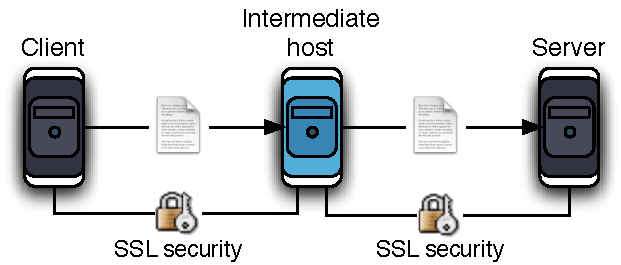
\includegraphics[scale=0.75]{tls-communication}
  \caption[Secure   communication  with  TLS]{Secure   communication  with
    Transport Layer Security (derived from \cite{mls}).}
  \label{fig:tls-communication}
\end{figure}

The  actual  communication between  the  client  and  the server  is  only
partially  secured. All  transmitted  messages can  be  accessed in  their
unencrypted version on the intermediate host.

In message-queue based  systems there is always at  least one intermediate
server --- the message-queue server.  This means that \gls{glo:TLS} cannot
be  used   to  provide  end-to-end  communication   security  between  the
distributed components.  But it can still be used to secure the individual
connections from each component to the message-queue server.

\subsection[Message Layer Security]{Message Layer Security (MLS)}
\label{sec:fundamentals:mls}

In  contrast   to  the   \emph{Transport  Layer  Security}   protocol  the
\emph{Message Layer Security} protocol  aims directly at the messages that
are sent between two systems (\cite{oasis-wss, mls}, MLS).

\gls{glo:MLS}  is  an  approach  that encapsulates  all  security  related
information within the transmitted message itself \cite{mls}. Securing the
message  instead  of the  transport  layer  has  several advantages.   The
following  list  is  based  on  the  information  that  can  be  found  in
\cite{mls}:

\begin{itemize}
\item \textbf{Increased  flexibility}. It  is possible to  secure selected
  parts of  a message  only \cite{mls}.  An  \gls{glo:MQS} has  to inspect
  received   messages   in   order   to   forward  it   to   the   correct
  destination. This part of the  message can be left unencrypted while the
  remaining part of the message is encrypted.
\item  \textbf{Extensibility}.  Intermediate systems  or services  can add
  their  own (signed) headers  to the  message without  breaking unrelated
  (\eg  encrypted) parts  of the  message. An  example that  is  listed in
  \cite{mls} is \emph{audit logging}.
\item \textbf{Support  for multiple protocols}. \gls{glo:MLS}  can be used
  to send messages securely over a  variety of protocols such as SMTP, FTP
  or  TCP  without relying  on  the  security  of the  transport  protocol
  \cite{mls}.
\end{itemize}

The  major strength of  \gls{glo:MLS} is  also its  greatest disadvantage.
Since the security information is integrated into the messages, the layout
of the  messages must  be known  to the security  layer. That  means, each
different message layout requires  an own implementation of \gls{glo:MLS}.
Another disadvantage is the complexity of this protocol which imposes some
overhead to the message processing step.

In  \cite{oasis-wss}  a  specification  for securing  \emph{Simple  Object
  Access  Protocol}  (SOAP)  messages  with \gls{glo:MLS}  can  be  found.
Figure~\ref{fig:mls-communication} depicts  the same communication problem
as Figure~\ref{fig:tls-communication},  \ie the communication  between two
systems with the usage of an intermediate host.

\begin{figure}[ht]
  \centering
  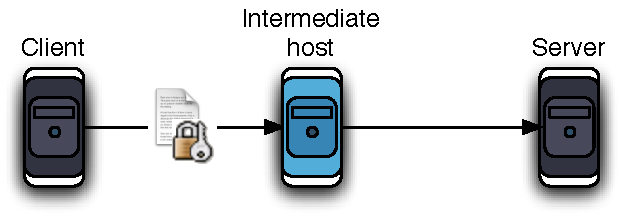
\includegraphics[scale=0.75]{mls-communication}
  \caption[Secure   communication  with  MLS]{Secure   communication  with
    Message Layer Security (based on the picture found in \cite{mls}).}
  \label{fig:mls-communication}
\end{figure}

The message is encrypted by the application running on the client host. In
contrast  to the  \gls{glo:TLS}, this  step is  performed only  once.  The
encrypted message is  sent to the intermediate host  and then forwarded to
its  final  destination.   Since  strong  cryptography  is  involved,  the
intermediate  host cannot  access (\ie  read) the  encrypted parts  of the
message.

Consequently  can \gls{glo:MLS}  be used  to provide  a  secure end-to-end
communication for distributed applications that use message-passing.


\subsection{Implications for the \gls{glo:XenBEE}}

The  previous sections  have shown  that only  the  \gls{glo:MLS} provides
secure  end-to-end  communication for  systems  that  use an  intermediate
message-queue server.   Authentication, as well as  strong cryptography is
in both protocols provided by a \emph{Public-Key Infrastructure}.

To  ensure   a  secure  communication   between  \emph{\gls{glo:xbe}}  and
\emph{\gls{glo:xbed}}  \emph{Message Layer  Security} has  to be  used. To
actually  make sure that  a client  ``talks'' to  correct server  and vice
versa, authentication  must be provided  in both directions.  This implies
that   the   \gls{glo:XenBEE}   uses   public-key   certificates   and   a
\gls{glo:PKI}.

% \section{Summary}

% This  section  summarize  the  technologies  that  will  be  used  in  the
% \gls{glo:XenBEE}.

% The \gls{glo:XenBEE} will use a message

%%% Local Variables: 
%%% mode: latex
%%% TeX-master: "main.tex"
%%% End: 
